\documentclass[12pt,a4paper]{article}
\usepackage[T1]{fontenc}
\usepackage[utf8]{inputenc}
\usepackage[brazil]{babel}
\usepackage{amsmath,amssymb}
\usepackage{geometry}
\usepackage{graphicx}
\usepackage{xcolor}
\usepackage{listings}
\usepackage{booktabs}
\usepackage{caption}
\usepackage{subcaption}
\usepackage{hyperref}
\usepackage{fancyhdr}
\usepackage{parskip}

\geometry{top=2.5cm,bottom=2.5cm,left=3cm,right=2.5cm}

\definecolor{codegreen}{rgb}{0,0.5,0}
\definecolor{codegray}{rgb}{0.5,0.5,0.5}
\definecolor{codeblue}{rgb}{0.1,0.1,0.7}
\definecolor{backcolour}{rgb}{0.97,0.97,0.97}

\lstdefinestyle{matlab}{
  language=Matlab,
  backgroundcolor=\color{backcolour},
  commentstyle=\color{codegreen},
  keywordstyle=\color{codeblue}\bfseries,
  numberstyle=\tiny\color{codegray},
  stringstyle=\color{orange!70!black},
  basicstyle=\ttfamily\footnotesize,
  breaklines=true,
  keepspaces=true,
  numbers=left, numbersep=6pt,
  frame=single, framerule=0.5pt,
  rulecolor=\color{gray!60},
  tabsize=4,
}

\pagestyle{fancy}
\fancyhf{}
\rhead{\small Processamento Digital de Imagens -- UFAM}
\lhead{\small Projeto \#6: \texttt{twodSFilter} \& \texttt{medianSFilter}}
\cfoot{\thepage}
\renewcommand{\headrulewidth}{0.4pt}

%==============================================================================
\begin{document}
%==============================================================================

\begin{center}
  {\Large\bfseries Universidade Federal do Amazonas}\\[4pt]
  {\large Disciplina: Processamento Digital de Imagens}\\[2pt]
  {\large Grupo de Pesquisa em Reconhecimento de Padrões e Otimização -- GPRP\&O}\\[12pt]
  \rule{\linewidth}{1.5pt}\\[6pt]
  {\LARGE\bfseries Projeto \#6}\\[4pt]
  {\Large\bfseries \texttt{twodSFilter} \& \texttt{medianSFilter}}\\[6pt]
  \rule{\linewidth}{1.5pt}\\[10pt]
  {\large Pedro Victor dos Santos Oliveira}\\[2pt]
  {\normalsize Manaus, \today}
\end{center}

\vspace{4mm}

%==============================================================================
\section{Objetivo}
%==============================================================================

Este projeto implementa duas funções de filtragem espacial 2-D em MATLAB:

\begin{enumerate}
  \item \textbf{\texttt{twodSFilter(f, w)}} — filtragem espacial linear
        (correlação 2-D) com padding replicado e normalização da entrada para
        $[0,1]$. Testada com filtro de média (\emph{box filter}) de tamanhos
        $3\times3$, $11\times11$ e $21\times21$ sobre a imagem
        \texttt{Fig\,3.37(a).jpg}.

  \item \textbf{\texttt{medianSFilter(f, w)}} — filtragem espacial pela
        mediana (operação não-linear) com padding replicado. Testada com
        vizinhança $3\times3$ sobre a mesma imagem.
\end{enumerate}

%==============================================================================
\section{Fundamentação Teórica}
%==============================================================================

\subsection{Filtragem Espacial Linear — Correlação 2-D}

A filtragem espacial linear de uma imagem $f(x,y)$ por um \emph{kernel}
$w(s,t)$ de tamanho $(2a+1)\times(2b+1)$ é definida pela operação de
correlação:

\begin{equation}
  g(x,y) = \sum_{s=-a}^{a} \sum_{t=-b}^{b} w(s,t)\, f(x+s,\; y+t)
  \label{eq:correlation}
\end{equation}

A convolução difere da correlação pelo sinal dos índices ($x-s$), mas para
kernels simétricos (como o filtro de média) as operações são equivalentes.

\subsection{Filtro de Média (\emph{Box Filter}) — Passa-Baixa}

O filtro de média utiliza um kernel cujos coeficientes são todos iguais:

\begin{equation}
  w_{n\times n} = \frac{1}{n^2}
  \begin{pmatrix}
    1 & 1 & \cdots & 1 \\
    \vdots & & & \vdots \\
    1 & 1 & \cdots & 1
  \end{pmatrix}_{n\times n}
  \label{eq:boxfilter}
\end{equation}

Este filtro atenua as altas frequências espaciais (transições abruptas de
intensidade), produzindo \textbf{suavização} (\emph{blurring}) da imagem.
Quanto maior o kernel, maior o grau de suavização, pois a janela de
integração engloba uma região espacial mais ampla.

Propriedades:
\begin{itemize}
  \item Remove ruído aditivo gaussiano, pois a média reduz a variância
        por um fator $n^2$.
  \item Borra bordas e detalhes finos — efeito indesejável em muitas
        aplicações.
  \item A \emph{resposta de frequência} é a função $\text{sinc}$ 2-D:
        altas frequências são fortemente atenuadas.
\end{itemize}

\subsection{Filtro de Mediana — Filtragem Não-Linear}

O filtro de mediana substitui cada pixel pelo valor mediano de sua
vizinhança $w\times w$:

\begin{equation}
  g(x,y) = \operatorname{mediana}\!\left\{\,f(x+s,\; y+t)
            \;\middle|\; s,t \in [-r, r]\,\right\},
  \quad r = \left\lfloor\tfrac{w}{2}\right\rfloor
  \label{eq:median}
\end{equation}

É uma operação \textbf{não-linear}: não pode ser expressa como
convolução/correlação. Suas propriedades incluem:

\begin{itemize}
  \item Excelente remoção de ruído impulsivo (\emph{salt-and-pepper}),
        pois valores extremos são descartados pelo ordenamento.
  \item Preservação de bordas melhor que o filtro de média.
  \item Menor suavização de regiões homogêneas em comparação com
        filtros lineares.
\end{itemize}

%==============================================================================
\section{Implementação}
%==============================================================================

\subsection{Função \texttt{twodSFilter.m}}

\lstinputlisting[style=matlab, caption={Função \texttt{twodSFilter.m} — filtragem linear 2-D comentada.}]{twodSFilter.m}

\subsection{Função \texttt{medianSFilter.m}}

\lstinputlisting[style=matlab, caption={Função \texttt{medianSFilter.m} — filtragem pela mediana comentada.}]{medianSFilter.m}

\subsection{Script Principal \texttt{main\_project6.m}}

\lstinputlisting[style=matlab, caption={Script principal de demonstração.}]{main_project6.m}

%==============================================================================
\section{Resultados}
%==============================================================================

\subsection{Imagem de Entrada}

A imagem \texttt{Fig\,3.37(a)} (Gonzalez \& Woods, \emph{Digital Image
Processing}, Cap.\ 3) é uma fotografia de uma placa de circuito impresso
(PCB) em tons de cinza ($455\times440$ pixels), com ruído
granular distribuído pela imagem. Essa imagem é classicamente utilizada
para demonstrar os efeitos de filtros espaciais.

\subsection{Filtro de Média — três tamanhos de kernel}

\begin{figure}[ht]
  \centering
  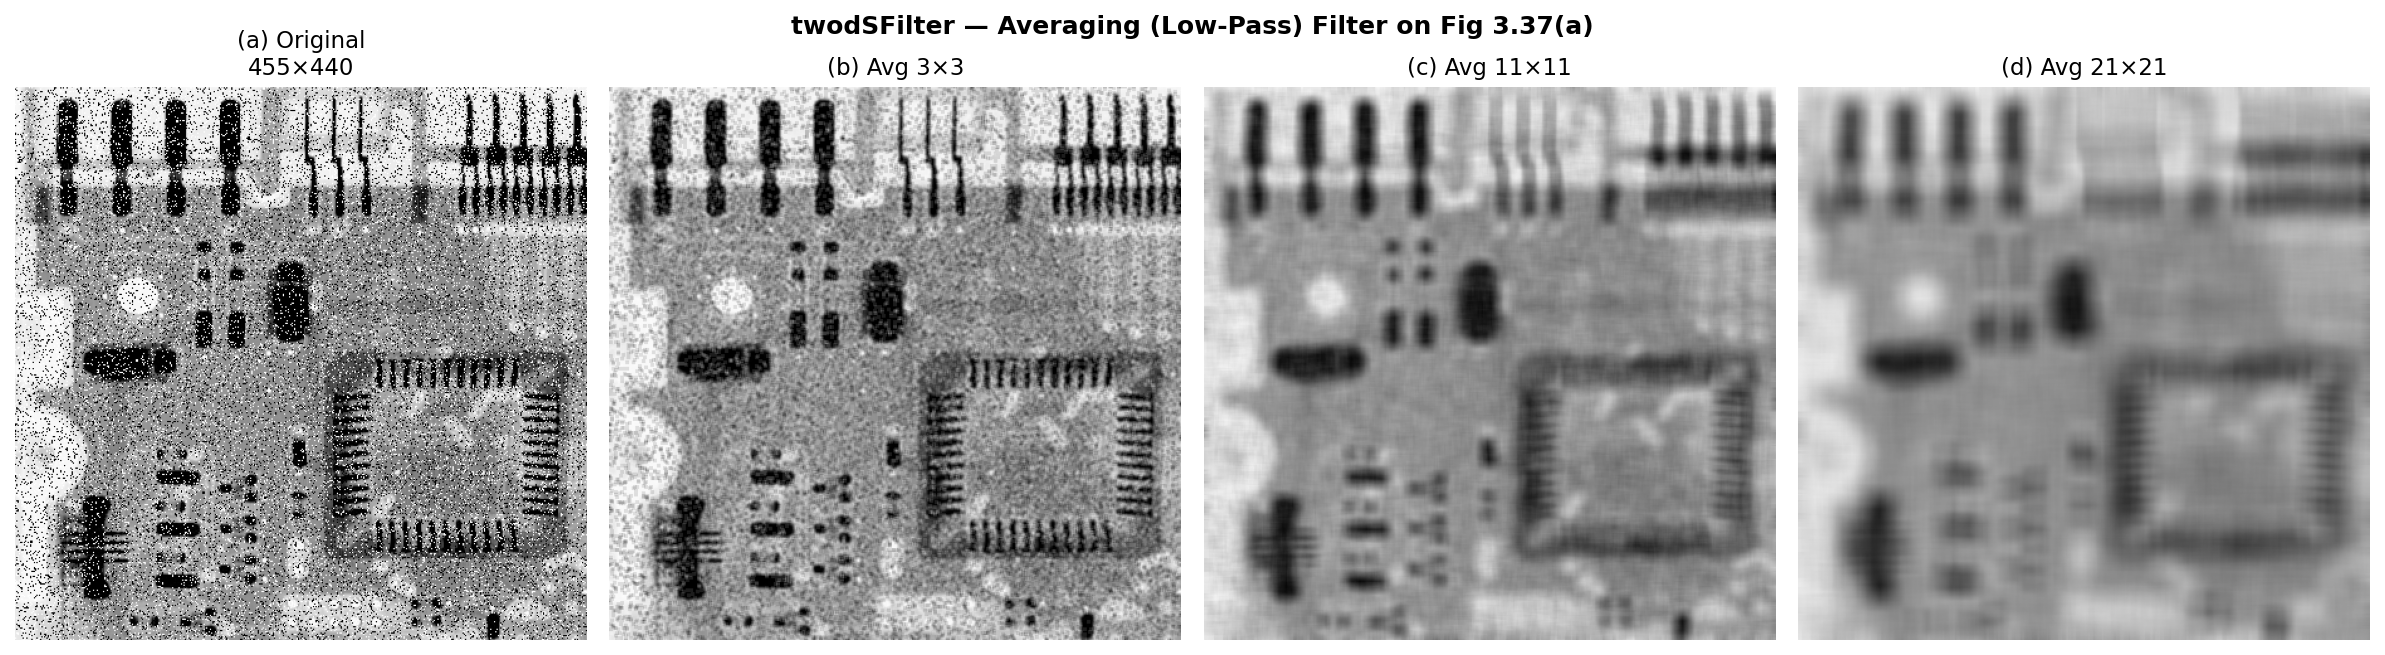
\includegraphics[width=\linewidth]{images/comparison_lowpass.png}
  \caption{Resultado da função \texttt{twodSFilter} com filtro de média
           para kernels $3\times3$, $11\times11$ e $21\times21$.
           O grau de suavização cresce com o tamanho do kernel.}
  \label{fig:avgfilter}
\end{figure}

Analisando a Figura~\ref{fig:avgfilter}:

\begin{itemize}
  \item \textbf{$3\times3$}: suavização leve; o ruído granular é levemente
        atenuado, mas os detalhes do circuito permanecem visíveis.
  \item \textbf{$11\times11$}: suavização moderada; o ruído é
        consideravelmente reduzido, mas bordas dos componentes começam a
        ser borradas.
  \item \textbf{$21\times21$}: suavização intensa; o ruído é praticamente
        eliminado, porém os detalhes finos (trilhas, pinos) ficam
        fortemente borrados — perda significativa de resolução espacial.
\end{itemize}

\subsection{Perfis de Intensidade}

\begin{figure}[ht]
  \centering
  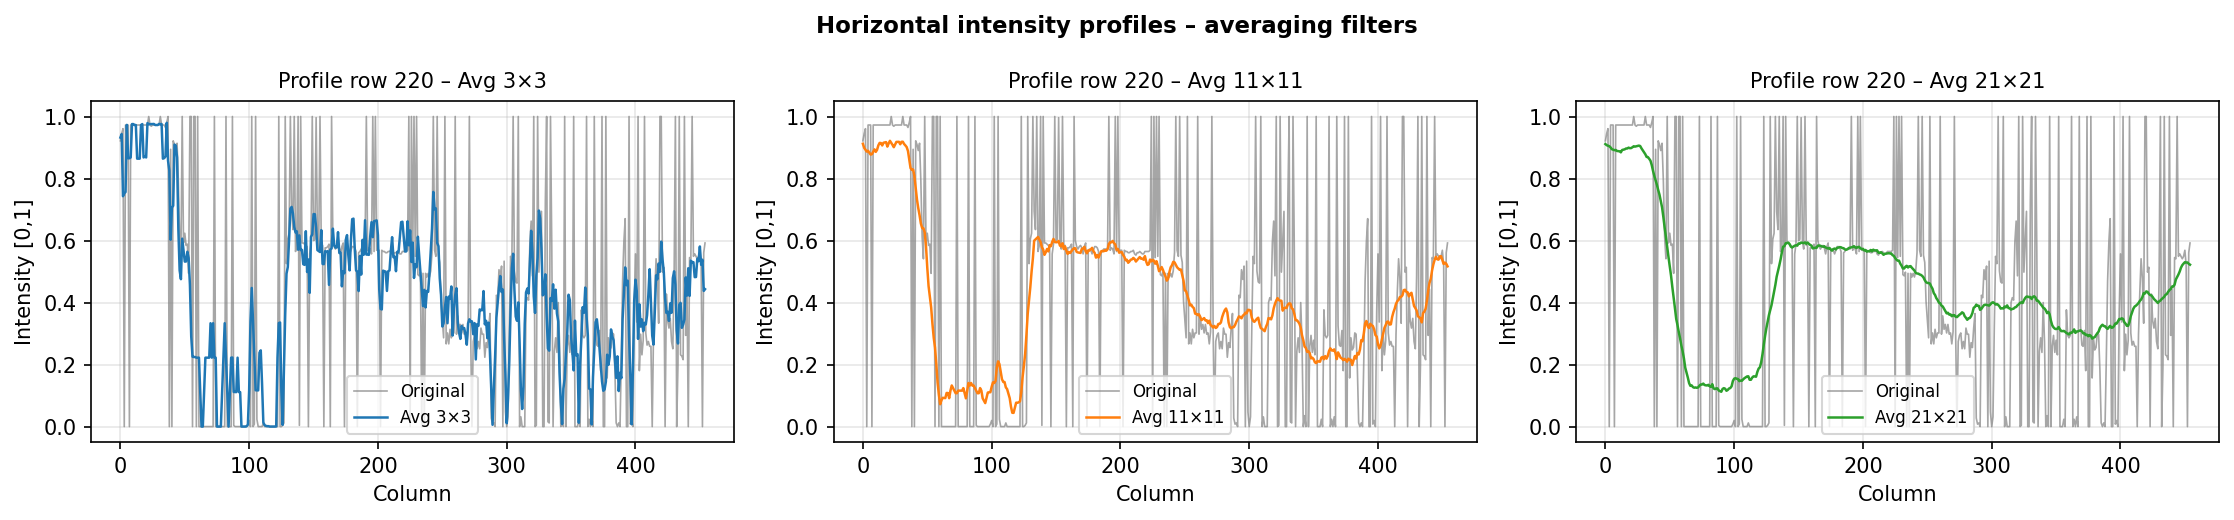
\includegraphics[width=\linewidth]{images/profiles.png}
  \caption{Perfis de intensidade horizontais (linha central da imagem)
           para os três kernels do filtro de média. A curva cinza é o
           original; a curva colorida é o resultado filtrado.}
  \label{fig:profiles}
\end{figure}

Os perfis da Figura~\ref{fig:profiles} confirmam que o filtro de média
atenua as oscilações de alta frequência (ruído) presentes no sinal original.
Com o kernel $21\times21$, as transições abruptas características das
bordas dos componentes eletrônicos são substancialmente suavizadas.

\subsection{Filtro de Mediana — $3\times3$}

\begin{figure}[ht]
  \centering
  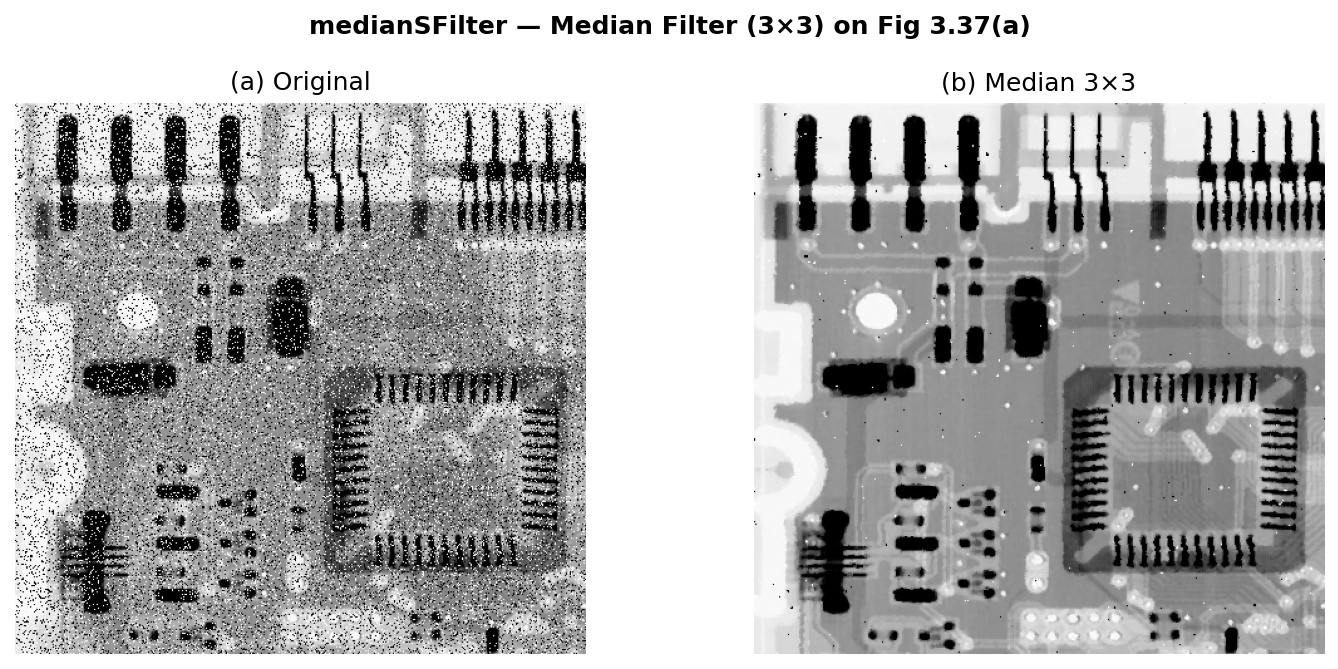
\includegraphics[width=0.75\linewidth]{images/comparison_median.png}
  \caption{Resultado da função \texttt{medianSFilter} com vizinhança
           $3\times3$. O ruído granular é reduzido enquanto as bordas
           dos componentes são melhor preservadas do que no filtro de
           média $3\times3$.}
  \label{fig:medfilter}
\end{figure}

\subsection{Comparação Geral}

\begin{figure}[ht]
  \centering
  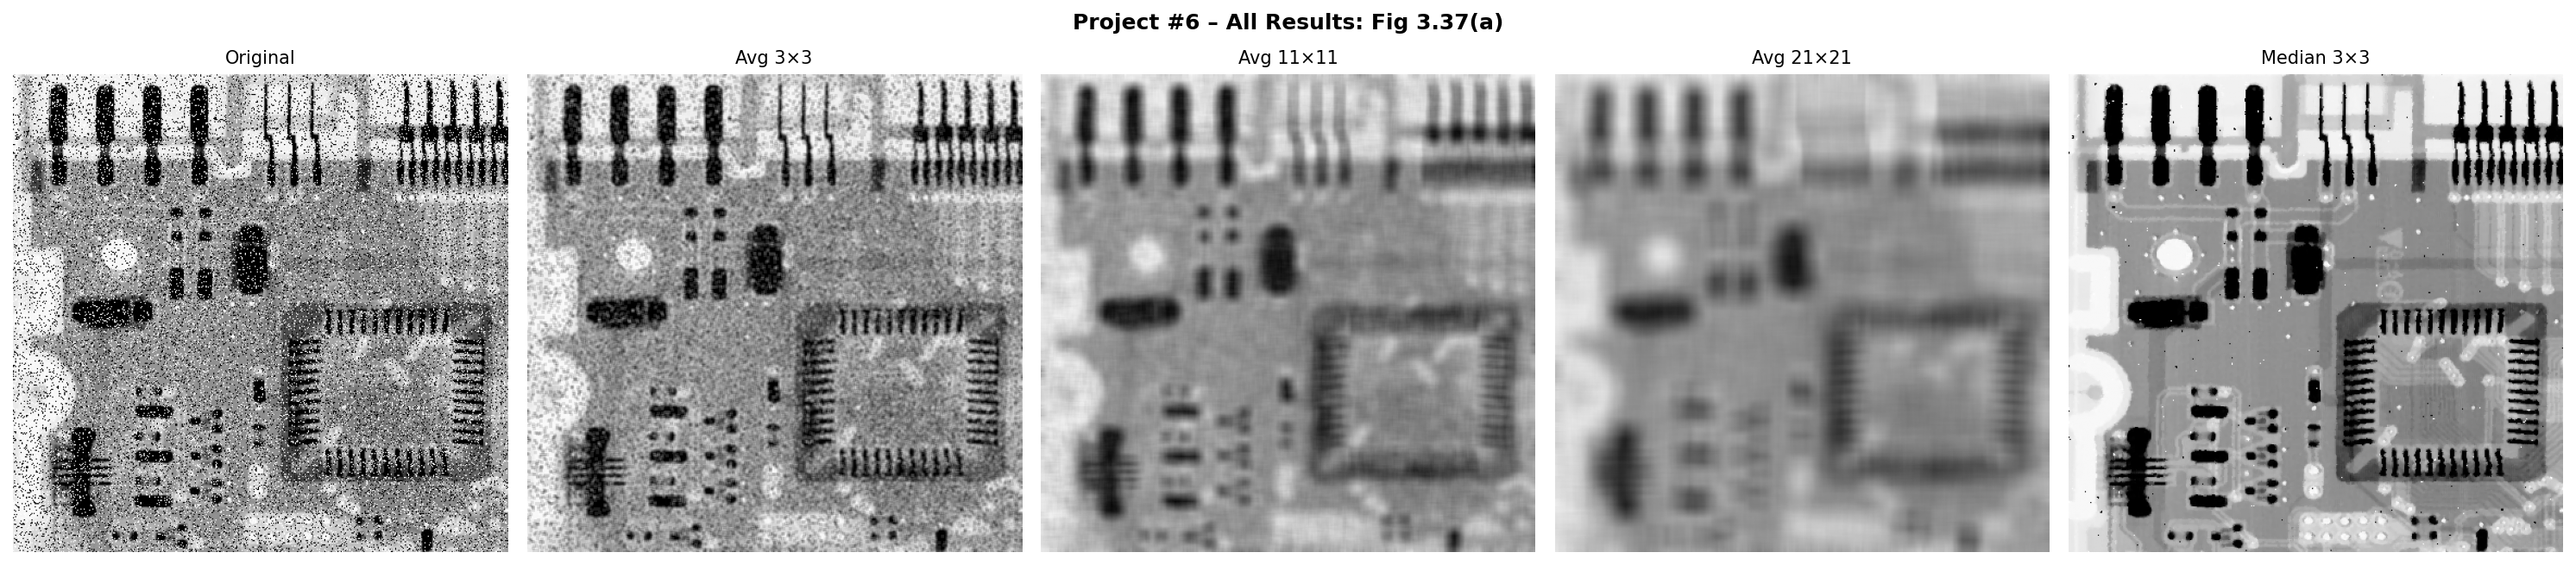
\includegraphics[width=\linewidth]{images/all_results.png}
  \caption{Todos os resultados lado a lado: original, três variantes do
           filtro de média e o filtro de mediana.}
  \label{fig:all}
\end{figure}

%==============================================================================
\section{Análise Comparativa}
%==============================================================================

\begin{table}[ht]
  \centering
  \caption{Comparação entre filtro de média e filtro de mediana.}
  \label{tab:compare}
  \begin{tabular}{lll}
    \toprule
    \textbf{Critério} & \textbf{Filtro de Média} & \textbf{Filtro de Mediana} \\
    \midrule
    Tipo de operação   & Linear (correlação) & Não-linear (ordenamento) \\
    Remoção de ruído gaussiano & Boa & Moderada \\
    Remoção de ruído impulsivo & Fraca & Excelente \\
    Preservação de bordas & Fraca (borra bordas) & Boa \\
    Custo computacional & $O(M N K^2)$ ops & $O(M N K^2 \log K)$ \\
    Efeito com kernel grande & Borrão progressivo & Segmentação por regiões \\
    \bottomrule
  \end{tabular}
\end{table}

A principal vantagem do filtro de mediana sobre o filtro de média é a
\textbf{preservação de bordas}: como o valor mediano pertence ao conjunto
de pixels da vizinhança, valores extremos (ruído impulsivo) são
descartados sem ``misturar'' intensidades de regiões diferentes. O filtro
de média, por sua vez, cria valores intermediários que suavizam
artificialmente as transições.

%==============================================================================
\section{Conclusão}
%==============================================================================

As funções \texttt{twodSFilter} e \texttt{medianSFilter} foram implementadas
e validadas sobre a imagem \texttt{Fig\,3.37(a)}:

\begin{itemize}
  \item \texttt{twodSFilter} implementa a correlação 2-D com padding
        replicado e normalização automática para $[0,1]$. Para o filtro
        de média, kernels maiores produzem maior suavização ao custo de
        borrar bordas e detalhes.
  \item \texttt{medianSFilter} implementa a filtragem pela mediana com
        padding replicado. É superior ao filtro de média na preservação
        de bordas e na remoção de ruído impulsivo.
  \item Ambas as funções reutilizam \texttt{imagePad4e} (Projeto \#4)
        para padding replicado, demonstrando reúso de código.
\end{itemize}

%==============================================================================
\section*{Referências}
%==============================================================================
\begin{itemize}
  \item GONZALEZ, R.~C.; WOODS, R.~E. \textit{Digital Image Processing},
        4ª~ed. Pearson, 2018. Cap.~3.
  \item GONZALEZ, R.~C.; WOODS, R.~E.; EDDINS, S.~L. \textit{Digital
        Image Processing Using MATLAB}, 3ª~ed. Gatesmark, 2020. Cap.~3.
  \item The MathWorks. \textit{conv2}, \textit{medfilt2} — MATLAB
        documentation. \url{https://www.mathworks.com/help/matlab/}.
\end{itemize}

\end{document}
